\pdfoutput=1
\documentclass[a4paper,pdftex]{article}

% ---Setting about the geometry of the document----
\usepackage{a4wide}
%\pagestyle{empty}

% ---Physics and Math Packages---
% \usepackage{amssymb,amsfonts,amsthm,mathtools}
% \usepackage{physics,braket,bm}

% ---underline---
\usepackage{ulem}

% ---Ignore the Warnings---
\usepackage{silence}
\WarningFilter{latexfont}{Some font shapes,Font shape}

% ---Insert the figure (If insert the `draft' at the option, the process becomes faster. And when you use pdflatex, add the option `pdftex' instead of `dvipdfmx`)---
\usepackage{graphicx}
\usepackage{caption,subcaption}

% ----Add a link to a text (When you use psflatex, add the option `pdftex' instead of `dvipdfmx` and turn of `pxjahyper')---
\usepackage{xcolor,hyperref}
\hypersetup{colorlinks=true,citecolor=orange,linkcolor=blue,urlcolor=magenta}
% \usepackage{pxjahyper}

% ---Tikz---
% \usepackage{tikz,pgf,pgfplots,circuitikz}
% \pgfplotsset{compat=1.15}
% \usetikzlibrary{intersections,arrows.meta,angles,calc,3d,decorations.pathmorphing}

% ---Add the section number to the equation, figure, and table number---
\makeatletter
   \renewcommand{\theequation}{\thesection.\arabic{equation}}
   \@addtoreset{equation}{section}
   
   \renewcommand{\thefigure}{\thesection.\arabic{figure}}
   \@addtoreset{figure}{section}
   
   \renewcommand{\thetable}{\thesection.\arabic{table}}
   \@addtoreset{table}{section}
\makeatother

% ---Index---
\usepackage{makeidx}
\makeindex 

% ---Title---
\title{PC Setup Manual}
\author{I. Miyane}
\date{\today}

\begin{document}

\maketitle

\begin{abstract}
  In this text, I will show you the overall introduction to writing the \LaTeX. It contains many topics, including how to install and set up, comfortable writing environments, packages, etc. I hope it would be helpful when I exchange the PC or someone familiar with me has some trouble.
\end{abstract}

\tableofcontents

\clearpage
\section{PC settings}

I will show you important settings when you get the new one in bullet points.

\begin{itemize}
  \item 
  Do the Updates, of course.

  \item   
  Check the Wi-Fi settings.
  \item 
  Install the following software:
  \begin{itemize}
    \item 
    Chrome
    
    \item 
    DeepL

    \item 
    Zoom

    \item 
    Tex Live
    
    \item 
    Python

    \item 
    VS Code

    \item 
    Zotero

    \item 
    Mathematica

    \item 
    Dropbox

    \item 
    Google Drive

    \item 
    Bing Wallpaper

  \end{itemize}

  \item 
  Set up the \uline{start up applications} by the following procedure:
  \begin{enumerate}
    \item 
    Press both [Windows key] + [R key] at the same time, and enter `\texttt{shell:startup}'. Then Startup folder will open.

    \item 
    Put the shortcut of the app file you want to register. If you cannot find the location of the app file, you should visit the start menu and do right-click on the app. Then you will access the app folder.

    \item 
    You can also open files or links. You just put the shortcut into the folder.

  \end{enumerate}

  \item 
  Uninstall \uline{One Drive}\footnote{
    I think it will be useful if I could master it.
  } \footnote{
    \uline{Do not} delete the One Drive folder in the User folder before transferring the important container such as the Desktop folder. If you cannot remove the One Drive folder, please try \href{https://www.pc-jozu.com/trouble/onedrive-file-delete/}{this web article}.
  }.

  \item 
  Turn off the touchpad when you use the PC mouse.

  \item 
  Set the \uline{Microsoft Edge} as the default PDF viewer\footnote{
    Although I have used \textit{Adobe Reader} as the PDF viewer, I come to think the \textit{Microsoft Edge} is far better than \textit{Adobe}.
  }:
  \begin{itemize}
    \item 
    Hide the bookmark bar.

    \item 
    Hide the taskbar from the settings.

  \end{itemize}
  
  \item 
  In the IME options, set spaces to half-width and do not update the conversion history.

  \item 
  Turn off the Notifications.

  \item 
  Sort out the Taskbar:
  \begin{itemize}
    \item 
    Command prompt

    \item 
    Control pannel

    \item 
    Task manger

    \item 
    Visual Studio Code

    \item 
    Zotero

    \item 
    Mathematica (if you can get it)

    \item 
    Chrome
    \item 
    DeepL

  \end{itemize}

  and settings are
  \begin{itemize}
    \item 




  \end{itemize}

  \item 
  Sort out the Desktop:
  \begin{itemize}
    \item 
    PC (or Windows Explorer)

    \item 
    User folder\footnote{Searching the setting for Desktop icon and check `Computer' and `User's folder'. The option is in the Theme settings at the Private option.}

    \item 
    (Personal folder)

    \item 
    Trash can
    
    \item 
    Dropbox

    \item 
    Google Drive

    \item 
    Downloads

    \item 
    Documents

    \item 
    Pictures

    \item 
    Music

    \item 
    Videos

    \item 
    archives (Google Drive)

    \item 
    reading\_list (Google Drive)

    \item 
    bibtex (Google Drive)\footnote{Change the icon from the property of the folder.}
    
  \end{itemize}

  and settings are
  \begin{itemize}
    \item 
    



  \end{itemize}

\end{itemize}

\section{Softwares}

\subsection{Chrome}

We should, anyway, install \uline{Chrome} at first. We will come to use Chrome mainly to download files from the Internet.

\begin{itemize}
  \item 
  Download the extended application, \uline{Click\&Clean} and \uline{Zotero Connector}, and display those applications and the Home Botton at the taskbar.[\ref{cc}]

  \begin{figure}[ht]
    \centering
    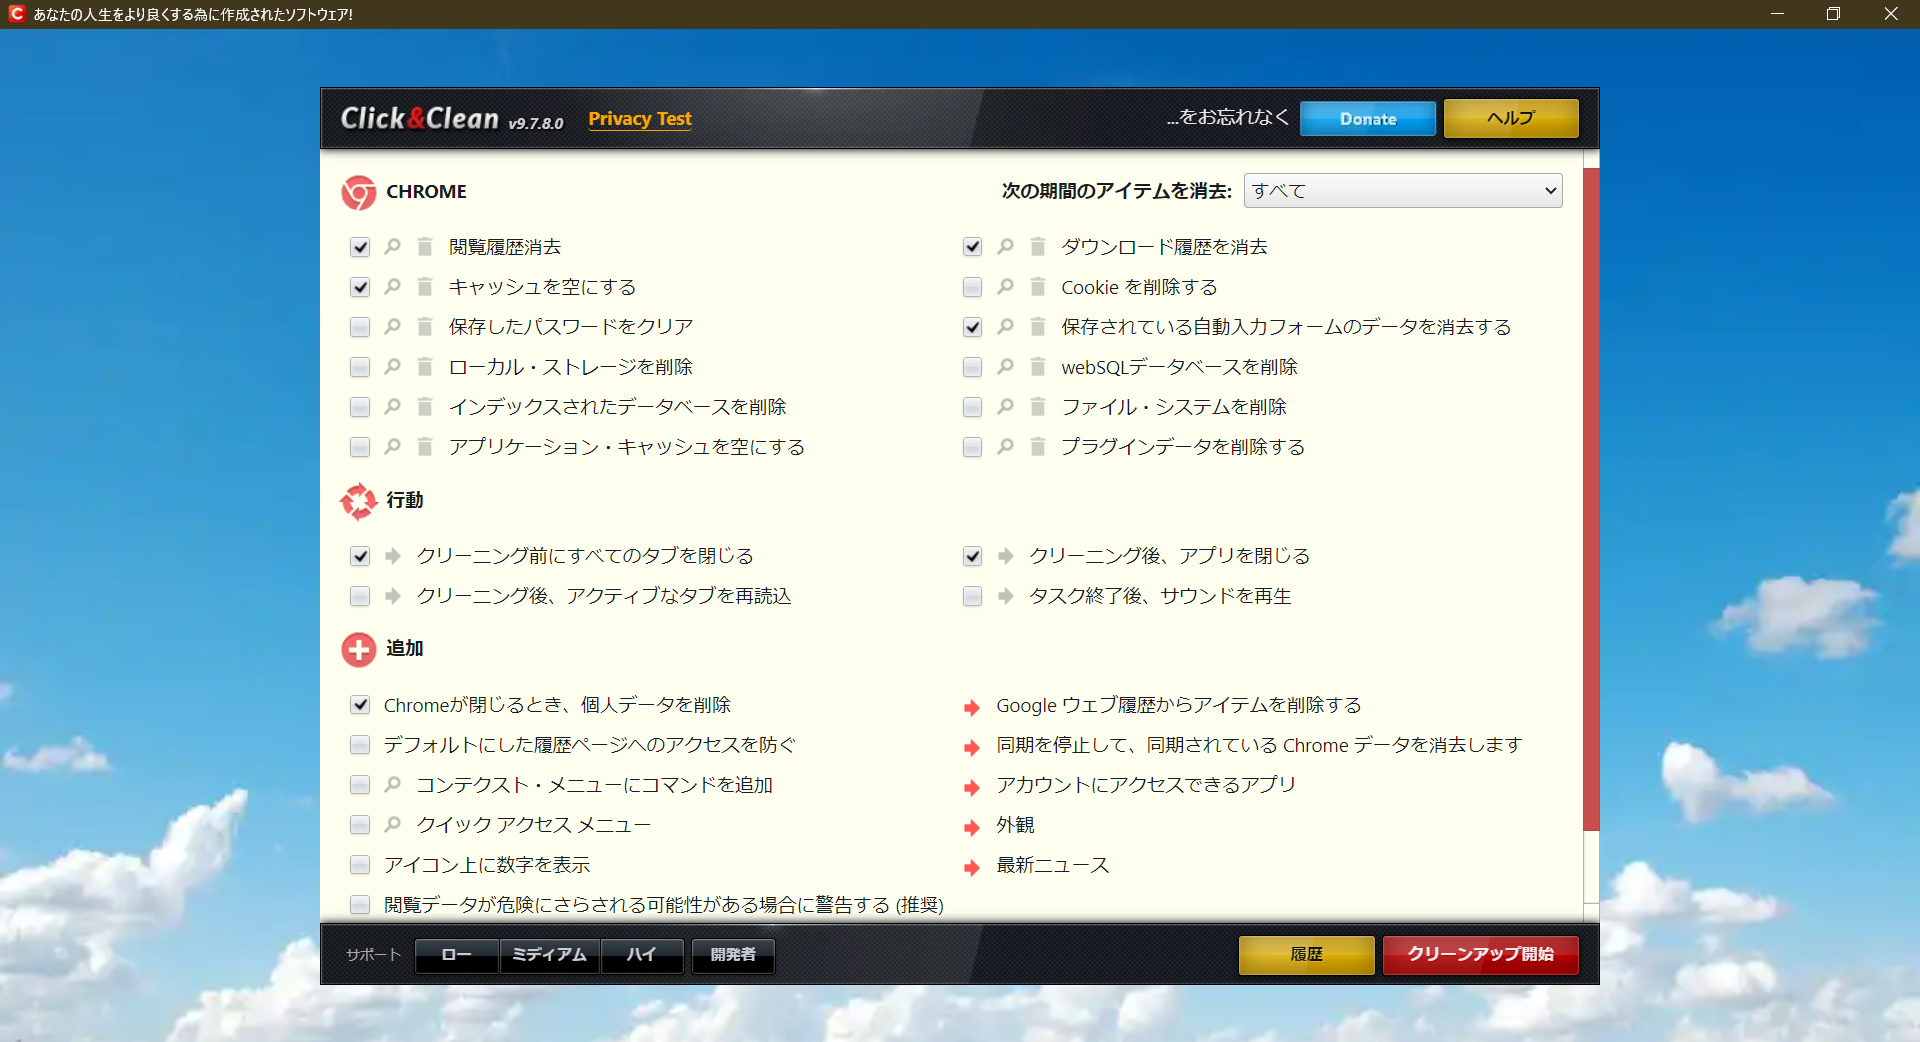
\includegraphics[width=0.8\columnwidth]{fig/ClickClean.png}
    \caption{settings of the Click\&Clean}
    \label{cc}
  \end{figure}

\end{itemize}

\subsection{Google Drive}

Getting the exe file from \href{https://www.google.com/intl/ja_jp/drive/download/}{here} and running it. We would use Google Drive to share the documents mainly. For the initial settings, the location of folders is difficult to treat for \LaTeX. Then, you should change the default location as follows:

\begin{enumerate}
  \item 
  Open the setting of Google Drive for Windows.

  \item 
  Check the ``Mirroring the files'' and specify the location of the file as \\ \texttt{C:/Users/itsuki.miyane}. In general, you cannot access the folders by your account because of the permission. So, by entering the folder and opening the property, you have to change the access permission of the folder.
  
\end{enumerate}

\subsection{Python}




\subsection{others}

\begin{itemize}
  \item 
  ffmpge (with AAC)

  \item 
  yt-dlp

  \item 
  TuneBrowser
  
\end{itemize}







\section{\LaTeX\ Setup manual}

There are two steps, generally speaking, to introducing the \LaTeX and its writing environment:

\begin{itemize}
  \item 
  Installing \LaTeX via \uline{Tex Live}.

  \item 
  Installing writing environments \uline{VS Code}, \uline{Zotero}, and setting up that software. 

\end{itemize}

\subsection{Installing \LaTeX}

This step is not difficult since the installer is already prepared. Go to \href{https://www.tug.org/texlive/acquire-netinstall.html}{this link} and get the installer (\href{https://mirror.ctan.org/systems/texlive/tlnet/install-tl-windows.exe}{install-tl-windows.exe}). Then just running the exe file, we finished installing the \LaTeX.  

\subsection{Set up for Zotero}

I think it is better to set up Zotero completely before setting up the VS Code. The order is not a crucial problem but it is preferable to finish the easier one for the fast. To write this section, I refer to the following articles:

\begin{itemize}
  \item 
  \href{https://qiita.com/shiro_takeda/items/dfb857e69aa8ed2cc977}{1}: To generate the citation key of Japanese books or articles.

  \item 
  \href{https://qiita.com/Yarakashi_Kikohshi/items/39dfbf3059aaf0690761}{2}: Brief introduction to synchronize the Zotero.

  \item 
  \href{https://necostat.hatenablog.jp/entry/2022/10/09/225731}{3}: More precise introduction than above one.

\end{itemize}

Citing the above articles, I set up the Zotero in the best way as far as I come up with. I assume that you have already installed Chrome.

\begin{enumerate}
  \item 
  Login to the Zotero account first.

  \item 
  Download Better BibTeX (BBT) from \href{https://retorque.re/zotero-better-bibtex/installation/}{here}. After downloading the XPI file, follow the instruction to install the BBT.

  \item 
  Download the Zotfile plugin from \href{https://github.com/jlegewie/zotfile/releases/download/v5.1.2/zotfile-5.1.2-fx.xpi}{here} and install it in the same way.

  \item 
  Move to the preference settings and set it up in the same way as the figure \ref{setting_zotero}\footnote{
    \textit{Citation key formula} is as follows:
    \begin{center}
      \texttt{auth+"\_"+title.splitIdeographs.select(1,2).capitalize+"\_"+year}
    \end{center}
  }.

  \item 
  Note that when you import a bib file, export from \textit{BBT} settings.

\end{enumerate}

\begin{figure}[ht]
  \begin{minipage}[ht]{0.19\columnwidth}
    \centering
    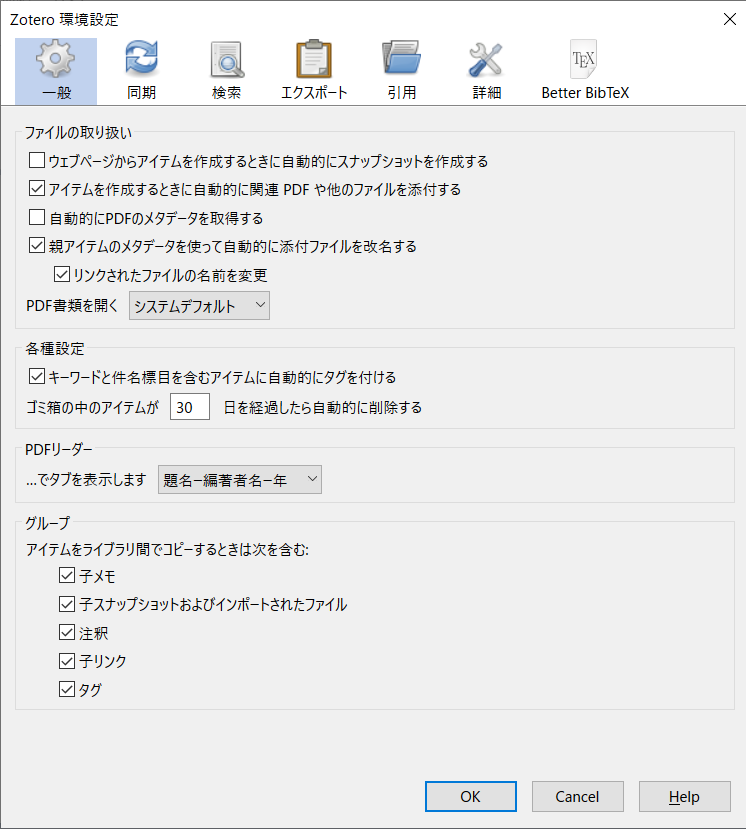
\includegraphics[width=\columnwidth]{fig/zotero01.png}
    \subcaption{setting 1}
  \end{minipage}
  \begin{minipage}[ht]{0.19\columnwidth}
    \centering
    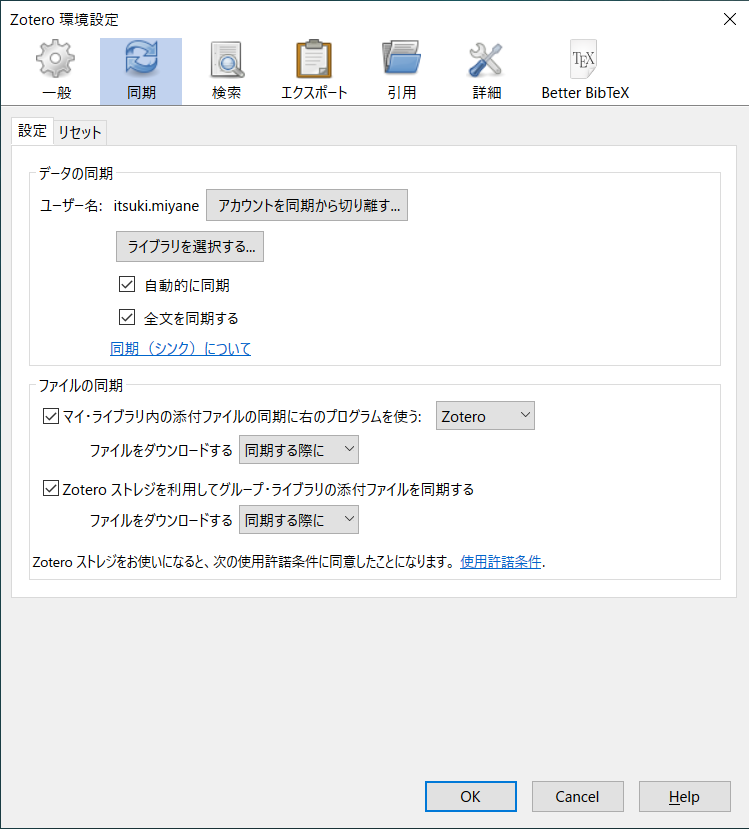
\includegraphics[width=\columnwidth]{fig/zotero02.png}
    \subcaption{setting 2}
  \end{minipage}
  \begin{minipage}[ht]{0.19\columnwidth}
    \centering
    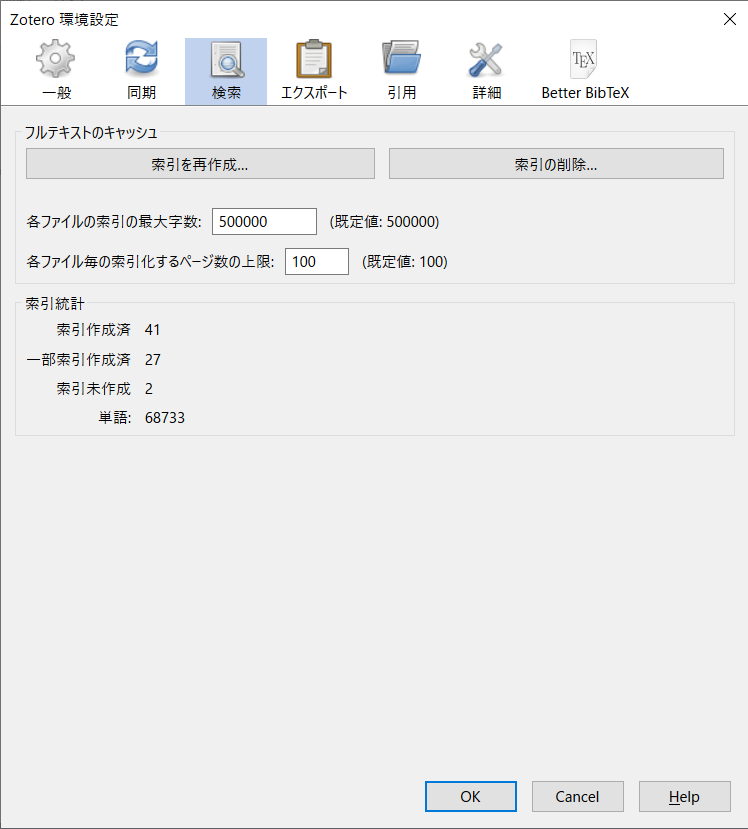
\includegraphics[width=\columnwidth]{fig/zotero03.png}
    \subcaption{setting 3}
  \end{minipage}
  \begin{minipage}[ht]{0.19\columnwidth}
    \centering
    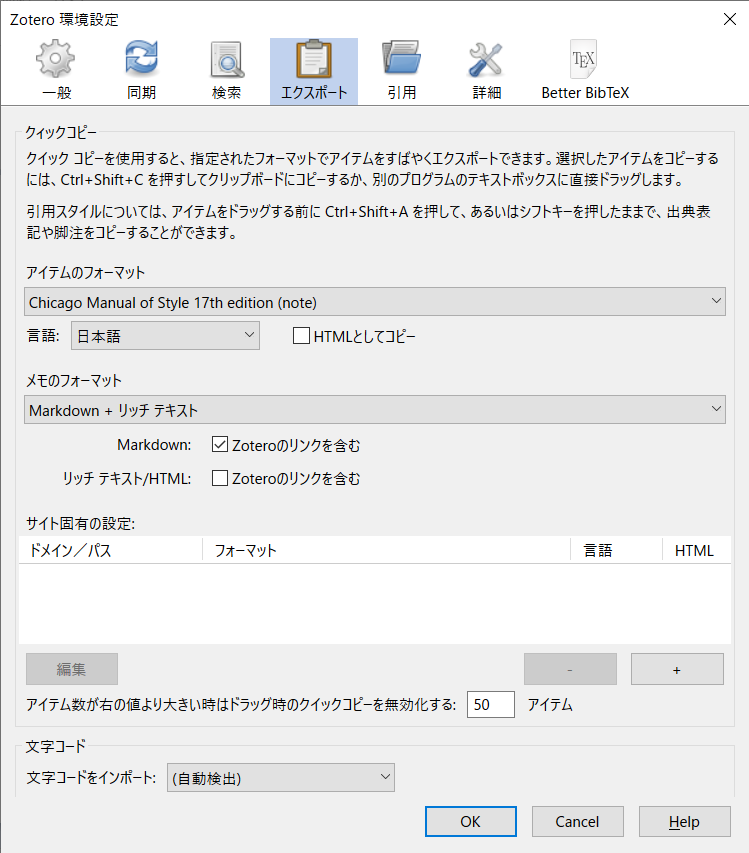
\includegraphics[width=\columnwidth]{fig/zotero04.png}
    \subcaption{setting 4}
  \end{minipage}
  \begin{minipage}[ht]{0.19\columnwidth}
    \centering
    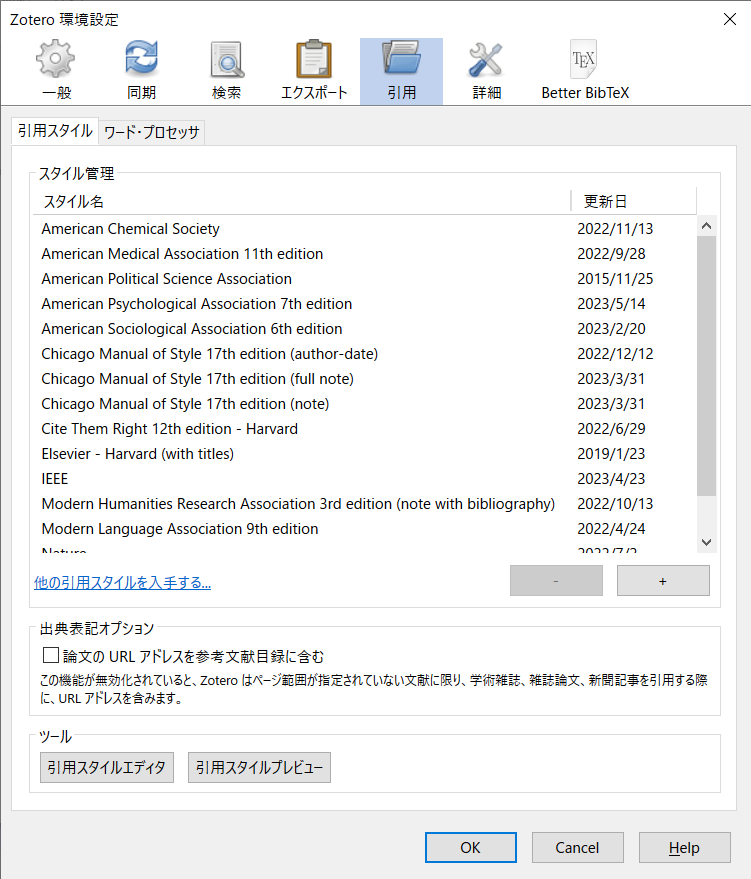
\includegraphics[width=\columnwidth]{fig/zotero05.png}
    \subcaption{setting 5}
  \end{minipage}
  \\
  \begin{minipage}[ht]{0.19\columnwidth}
    \centering
    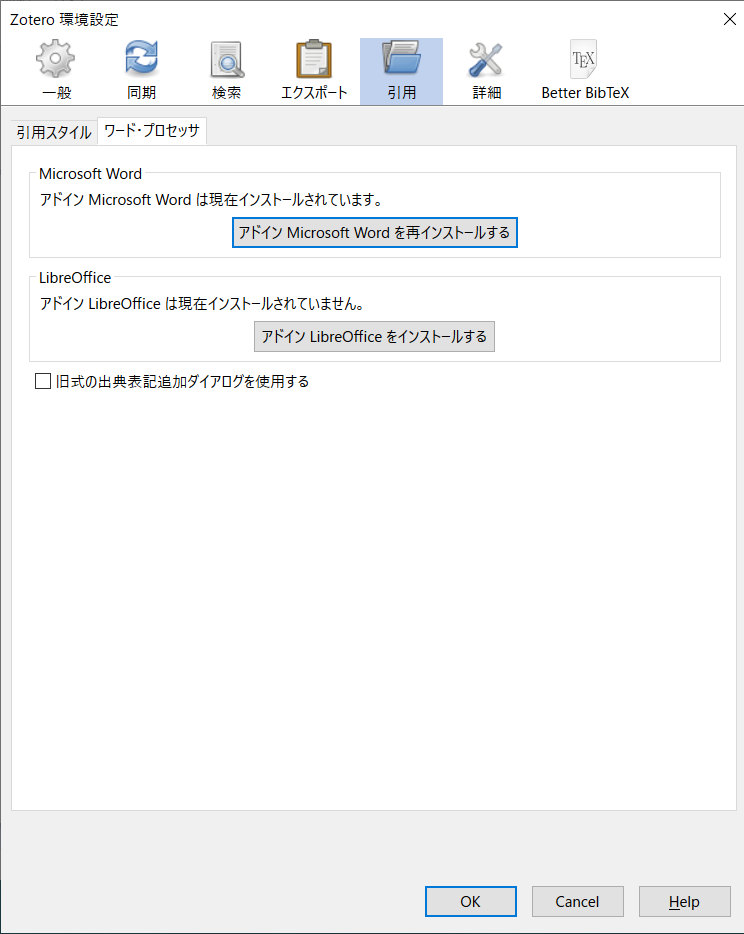
\includegraphics[width=\columnwidth]{fig/zotero06.png}
    \subcaption{setting 6}
  \end{minipage}
  \begin{minipage}[ht]{0.19\columnwidth}
    \centering
    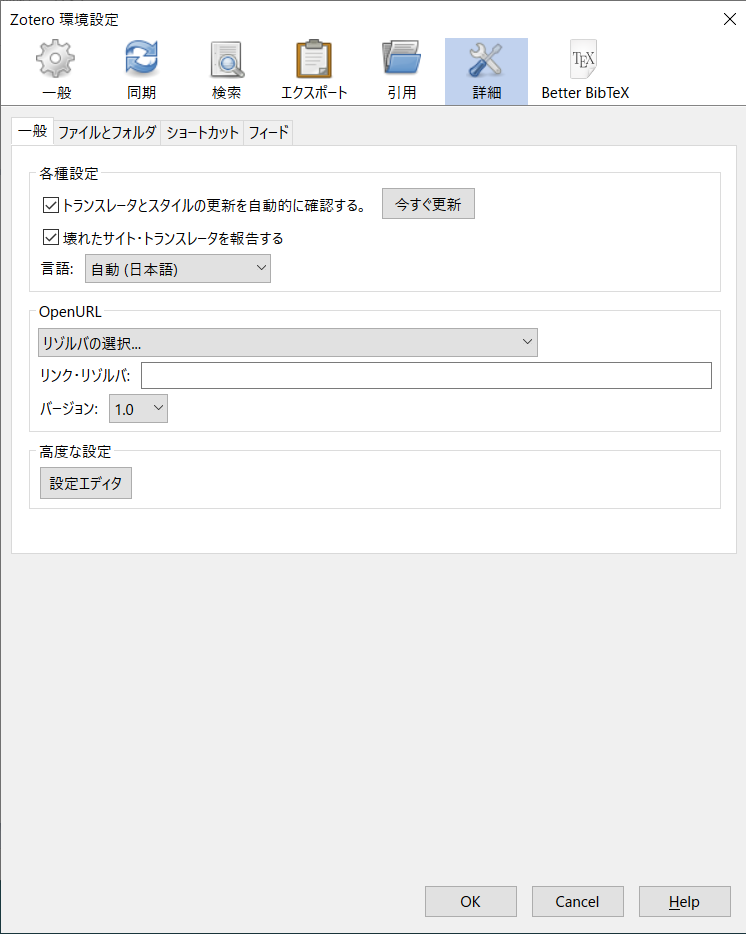
\includegraphics[width=\columnwidth]{fig/zotero07.png}
    \subcaption{setting 7}
  \end{minipage}
  \begin{minipage}[ht]{0.19\columnwidth}
    \centering
    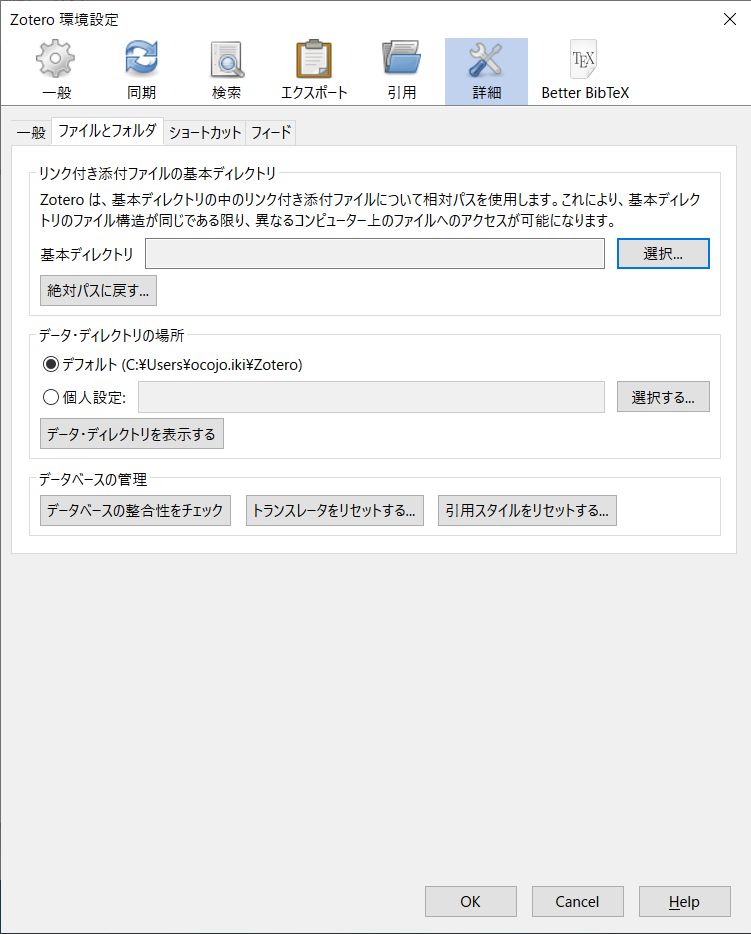
\includegraphics[width=\columnwidth]{fig/zotero08.png}
    \subcaption{setting 8}
  \end{minipage}
  \begin{minipage}[ht]{0.19\columnwidth}
    \centering
    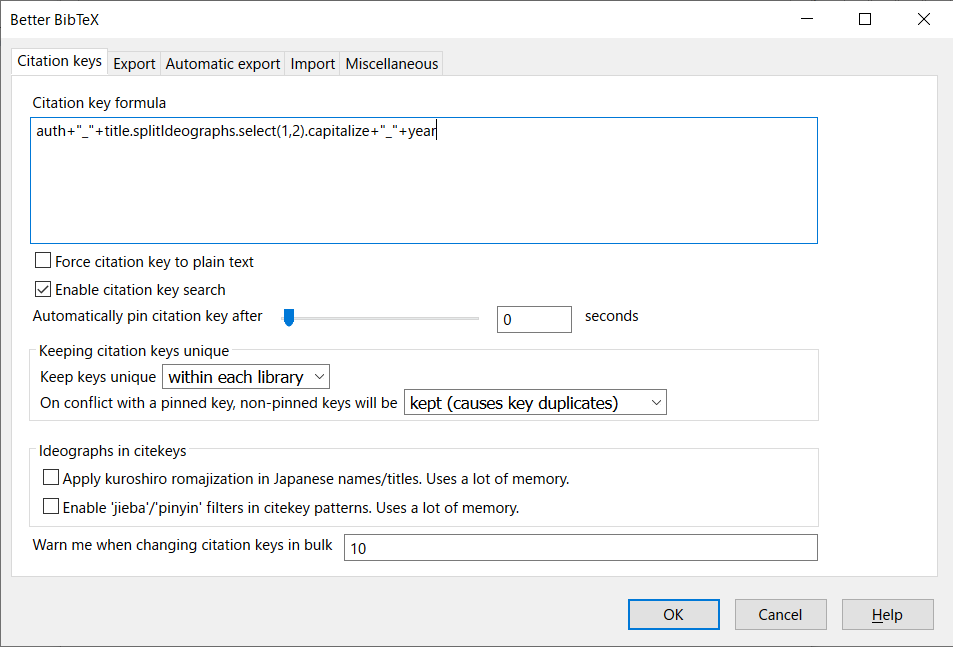
\includegraphics[width=\columnwidth]{fig/zotero09.png}
    \subcaption{setting 9}
  \end{minipage}
  \begin{minipage}[ht]{0.19\columnwidth}
    \centering
    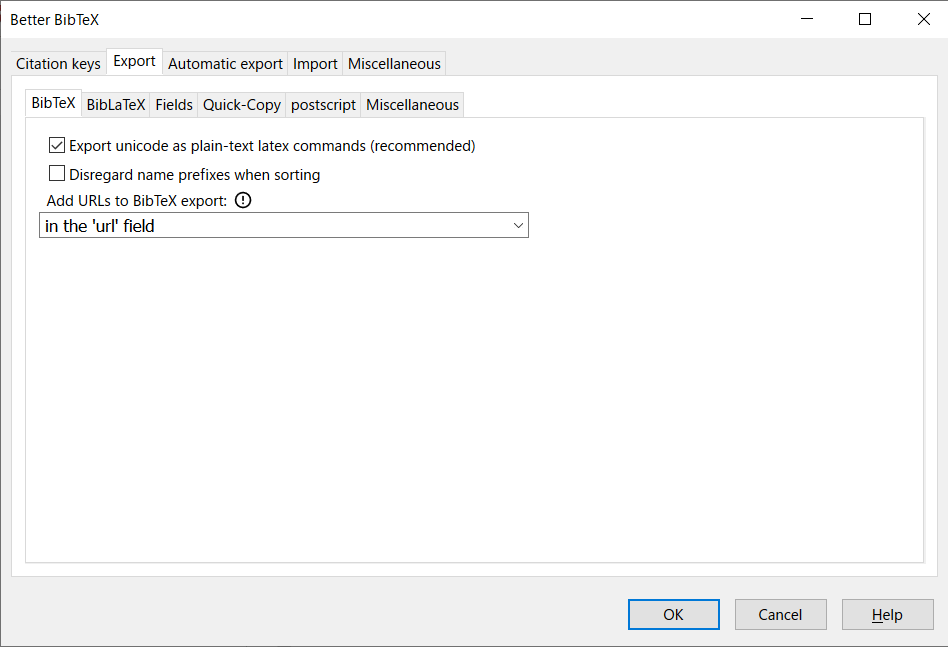
\includegraphics[width=\columnwidth]{fig/zotero10.png}
    \subcaption{setting 10}
  \end{minipage}
  \\
  \begin{minipage}[ht]{0.19\columnwidth}
    \centering
    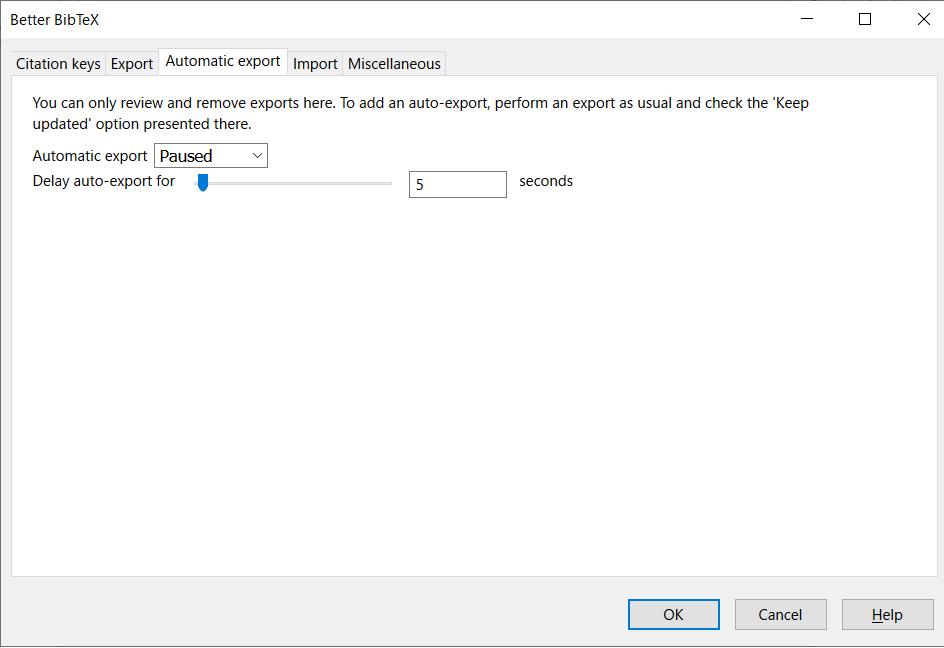
\includegraphics[width=\columnwidth]{fig/zotero11.png}
    \subcaption{setting 11}
  \end{minipage}
  \begin{minipage}[ht]{0.19\columnwidth}
    \centering
    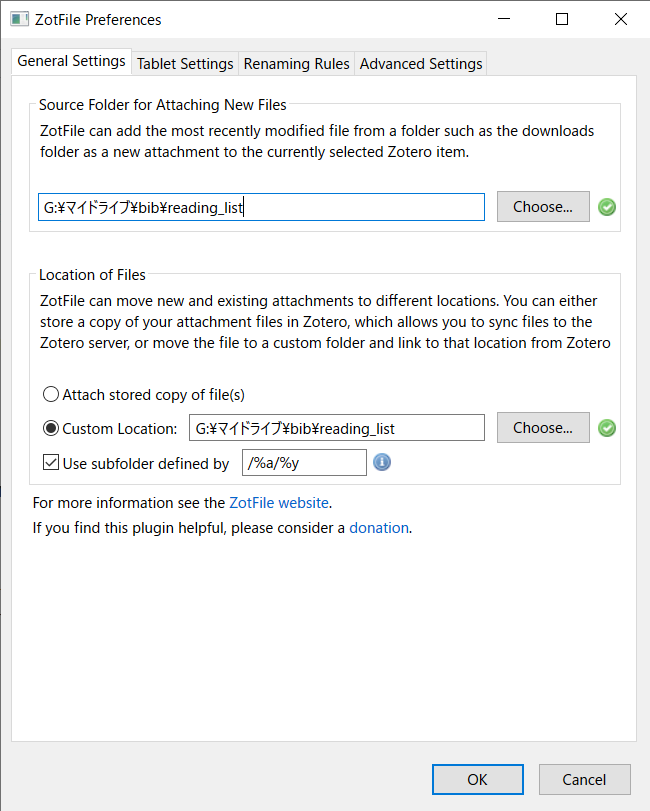
\includegraphics[width=\columnwidth]{fig/zotero12.png}
    \subcaption{setting 12}
  \end{minipage}
  \begin{minipage}[ht]{0.19\columnwidth}
    \centering
    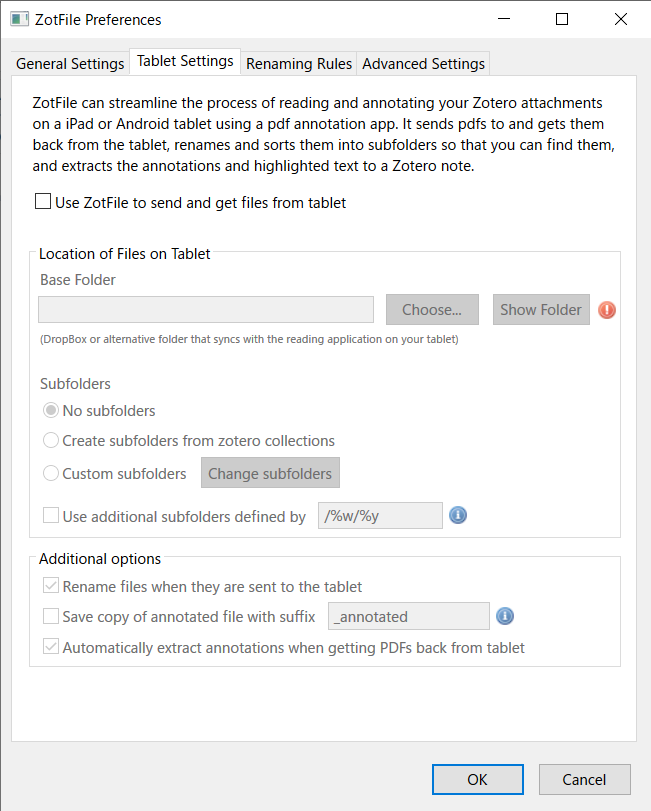
\includegraphics[width=\columnwidth]{fig/zotero13.png}
    \subcaption{setting 13}
  \end{minipage}
  \begin{minipage}[ht]{0.19\columnwidth}
    \centering
    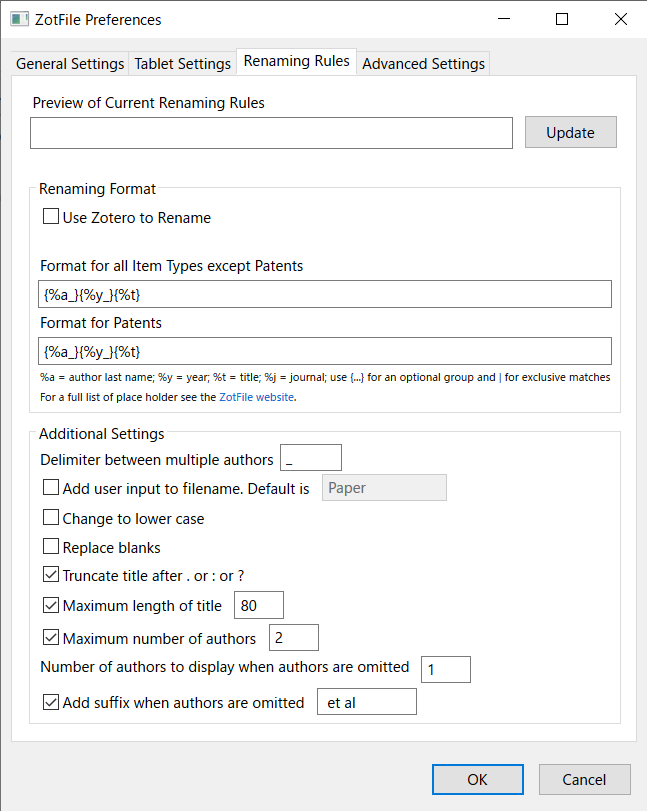
\includegraphics[width=\columnwidth]{fig/zotero14.png}
    \subcaption{setting 14}
  \end{minipage}  
  \begin{minipage}[ht]{0.19\columnwidth}
    \centering
    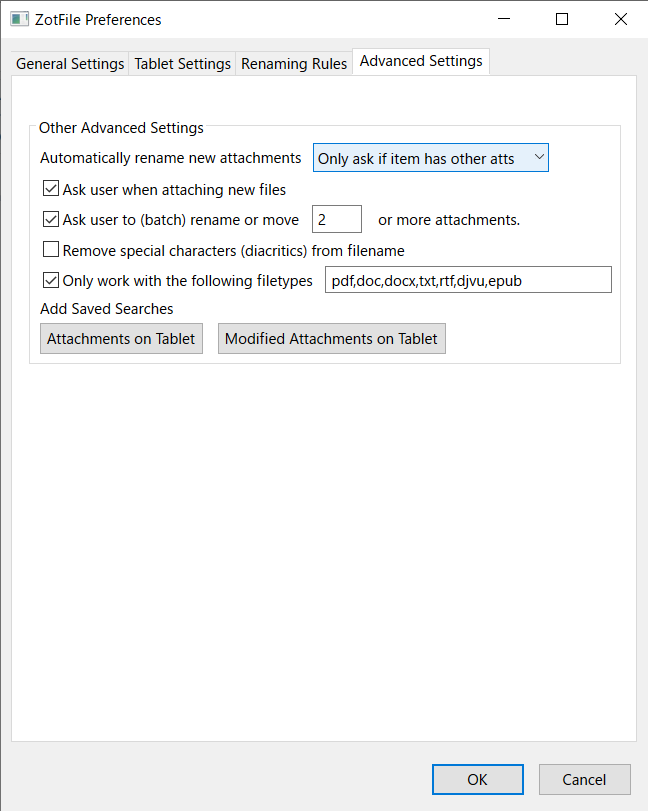
\includegraphics[width=\columnwidth]{fig/zotero15.png}
    \subcaption{setting 15}
  \end{minipage}
  \caption{Setting of Zotero}
  \label{setting_zotero}
\end{figure}

That's all about Zotero!


\subsection*{Edit on December 10, 2023}

We should add the additional options.

\begin{itemize}
  \item 
  Disable auto-produced tags.
  \item 
  Ignore fields (Export->Fields->Fields to omit from export: file,abstract,month)
\end{itemize}


\subsection{Set up for VS Code}

It is useful to use VS Code to write tex texts. 

\begin{enumerate}
  \item 
  To synchronize VS Code settings, you just log in to the Microsoft account.

  \item 
  Turn on the Grammarly. I cited \href{https://qiita.com/simonritchie/items/f49943f08cd09b92f3f9}{here}. 

\end{enumerate}

List of shortcuts:

\begin{itemize}
  \item 
  Command Palet: \texttt{[Ctrl]+[Shift]+[P]}

  \item 
  Settings: \texttt{[Ctrl]+[,]} \\
  Click the above button, you can open the settings.json.

\end{itemize}

\subsubsection{settings.json}

Now, I told you the bad news. It is that I cannot prepare the complete settings.json which allows us to compile any tex files automatically. I mean we should adjust the json file to the compile method each time. It is avoidable by using the latexmk but I think this way is faster than the way latexmk as a result, and this way is also fun for me. Here, I listed up some examples of the settings:

\begin{itemize}
  \item 
  \uline{pdflatex}

  In English, pdflatex seems to be very familiar to researchers. You should remember that compile twice when you use hyperref. So, the recipe becomes

    \texttt{"pdflatex",} \phantom{.} \\
    \texttt{"pdflatex",} .
  
  It's not complex. If you want to use bibtex or mendex, you should compile the tex file once and execute the command that you want. After that, compile pdflatex twice. That recipe becomes

    \texttt{"pdflatex",} \phantom{.} \\
    \texttt{"bibtex",} \phantom{.} \\
    \texttt{"mendex",} \phantom{.} \\
    \texttt{"pdflatex",} \phantom{.} \\
    \texttt{"pdflatex",} .
  
  \item 
  \uline{upLaTex}

  There exists, of course, unavoidable situations I have to write in Japanese. Use upLaTex in such a situation. Unlike pdflatex I mentioned above, upLaTex generates a dvi file. So, there is more extra step, dvipdfmx. Here is a full compilation:

    \texttt{"upLaTex",} \phantom{.} \\
    \texttt{"bibtex",} \phantom{.} \\
    \texttt{"mendex",} \phantom{.} \\
    \texttt{"upLaTex",} \phantom{.} \\
    \texttt{"upLaTex",} \phantom{.} \\
    \texttt{"upLaTex",} .

\end{itemize}

They are examples of the contents of the json file. Editing the recipe of the json file flexibly, enjoy the \TeX\ life!

\subsubsection{citation}

Here are references:
\begin{itemize}
  \item 
  \href{https://qiita.com/passive-radio/items/623c9a35e86b6666b89e}{This} is the complete setting guide. After you just follow this instruction, your \LaTeX\ life becomes far better!

  \item 
  \href{https://qiita.com/K-eno/items/53b81b4501f1f8318fa4}{This} is the supplemental but very useful. You should read this article when you are free at least once.
  
\end{itemize}

\subsubsection{Font family}

After downloading the Japanese language package, you should install the Font from \href{https://github.com/mzyy94/RictyDiminished-for-Powerline}{here}. 

\subsubsection{GitHub Pages}

Reference is \href{https://miya-system-works.com/blog/detail/vscode-github/}{here}.

(I will update GitHub Pages...)





\section{In writing \LaTeX}

\subsection{packages}

\begin{itemize}
  \item 
  article or jsarticle: in English or Japanese

  \item 
  silence: ignore the Warnings

  \item 
  amssymb, amsfonts, amsthm, mathtools: math

  \item 
  physics, braket, bm: physics

  \item 
  tcolorbox$\rightarrow$ to surround the paragraph

  \item 
  \texttt{\texorpdfstring{TEXstring}{PDFstring}}
  $\rightarrow$
  using the mathematical symbols at the section title even if you use the \texttt{hyperref}

\end{itemize}

\subsection{WSL}

I heard I will be able to compile far faster in virtualized environments and I wanted to try to construct it. Let me show the procedure:
\begin{enumerate}
  \item 
  Start command prompt and enter ``\texttt{start powershell}'' to open the Powershell.
  \item 
  Install WSL by entering ``\texttt{wsl --install}'', just do this.
  \item 
  Restart PC and start Ubuntu from the start menu.
  \\
  You will be asked the username and password. I have set as followings:
  \begin{itemize}
    \item 
    username: imiya
    ,
    \item 
    password: miyA2000
    .
  \end{itemize}
  After finishing setups, update the Ubuntu by \texttt{\$ sudo apt -y update}. (You will be asked password again.)
  \item 
  Install TexLive to Ubuntu. Enter \texttt{\$ sudo apt-get install texlive-full} and start installing. It may take tens of minutes, so I want to beg your patience.
  \item
  If there are something wrong about fonts, run \\
  \texttt{\$ sudo kanji-config-updmap-sys haranoaji} to set japanese default fonts.
  \item 
  Run \texttt{\$ sudo apt install evince poppler-data} to install the external PDF viewer.
  \item 
  Register the bst files by following procedure:
  \begin{itemize}
    \item 
    Move to \texttt{/usr/share/texlive/texmf-dist/bibtex/bst/base}. (I think any location is fine as long as it is under the bibtex directory.)
    \item 
    Put the \texttt{ytphys.bst}.
    \item 
    Run \texttt{mktexlsr} with \texttt{sudo}.
  \end{itemize}
\end{enumerate}
(I mainly referred \href{https://zenn.dev/minatoneko/articles/b4038eb6524199}{this web article}.)

\subsection{bst files}

BST files define the appearance of the output you cited. If you get the BST file you prefer, go to the directory \texttt{(C:/)texlive/texmf-local/bibtex/bst/local} and put there the files. After copying the files, \uline{make sure to run the command \texttt{mktexlsr}} to load the BST file in the computer. If you complete the settings about Zotero, you can cite the reference as \index{AGT correspondence@AGT correspondence}\cite[AGT]{Alday_LiouvilleCorrelation_2010}. I have also appended an index.

\subsection{Tips}

\begin{itemize}
  \item 
  If hyperref refers to the wrong parts, review the numbering rules at the preamble. 




\end{itemize}


\clearpage
\bibliography{bib}
\bibliographystyle{ytphys}

\clearpage
\printindex

\end{document}
